% gc-15-Taylor.tex

\documentclass[xcolor=dvipsnames]{beamer}
\usepackage{teachbeamer}

\title{Maclaurin and Taylor Series}
\subtitle{{\CourseNumber}, BCIT}

\author{\CourseName}

\date{April 24, 2018}

\begin{document}

\begin{frame}
  \titlepage
\end{frame}

\begin{frame}
  \frametitle{Sequences and Series}
  \begin{block}{Infinite Sequence}
    An infinite sequence is a function whose
    domain is the set of positive integers.
  \end{block}
Here is an example: $a(n)=2n$ for $n=1,2,3,\ldots$. We usually write
$a_{n}$ instead of $a(n)$. The infinite sequence is $2,4,6,\ldots$.
The infinite sequence itself is often called $(a_{n})_{n\in\mathbb{N}}$.
\begin{block}{Infinite Series}
  Given an infinite sequence $a_{n}$, the infinite series $s_{n}$ is
  an infinite sequence defined as follows: $s_{n}=a_{1}+a_{2}+\ldots{}+a_{n}$.
\end{block}
$s_{n}$ is called a partial sum of the sequence
$(a_{n})_{n\in\mathbb{N}}$. It is often written as
\begin{equation}
  \label{eq:tahxooke}
  s_{n}=\sum_{i=1}^{n}a_{i}
\end{equation}
\end{frame}

\begin{frame}
  \frametitle{Convergence and Divergence}
  \begin{description}
  \item[converges] $(a_{n})_{n\in\mathbb{N}}$ converges to the real
    number $L$ if for every positive real number $\varepsilon$ there
    exists an integer $N$ such that for all $n>N$ it is true that
    $\vert{}a_{n}-L\vert{}<\varepsilon$. $L$ is the \alert{limit} of
    this sequence.
  \item[diverges] $(a_{n})_{n\in\mathbb{N}}$ diverges if no limit
    exists. $(a_{n})_{n\in\mathbb{N}}$ diverges to positive infinity
    $\infty$ if for every real number $M$ there is an integer $N$ such
    that for all $n$ larger than $N$ it is true that $a_{n}>M$. We say
    $\lim_{n\rightarrow\infty}a_{n}=\infty$ or
    $a_{n}\longrightarrow\infty$. $(a_{n})_{n\in\mathbb{N}}$ diverges
    to negative infinity $-\infty$ if for every real number $m$ there
    is an integer $N$ such that for all $n$ larger than $N$ it is true
    that $a_{n}<m$. We say $\lim_{n\rightarrow\infty}a_{n}=-\infty$ or
    $a_{n}\longrightarrow{}-\infty$.
  \end{description}
\end{frame}

\begin{frame}
  \frametitle{Geometric Series}
  \alert{Geometric series} have the form
  \begin{equation}
    \label{eq:ahngahph}
    s_{n}=a+ar+ar^{2}+\ldots{}+ar^{n-1}
  \end{equation}
  The notation for the limit is as follows,
  \begin{equation}
    \label{eq:eeyengog}
    \lim_{n\rightarrow\infty}s_{n}=\sum_{n=1}^{\infty}ar^{n-1}
  \end{equation}
$r$ is called the \alert{ratio} of the geometric series. Subtract
$s_{n}-rs_{n}$ to find out that
\begin{equation}
  \label{eq:seciefai}
  \sum_{n=1}^{\infty}ar^{n-1}=\frac{a}{1-r}\mbox{ for }\vert{}r\vert{}<1
\end{equation}
If $\vert{}r\vert{}\geq{}1$ then the limit does not exist.
\end{frame}

\begin{frame}
  \frametitle{Geometric Series}
  \begin{figure}[h]
    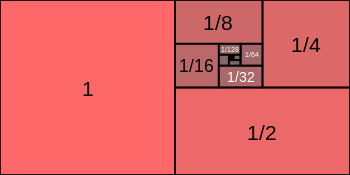
\includegraphics[scale=0.7]{./diagrams/geoser.png}
  \end{figure}
\end{frame}

\begin{frame}
  \frametitle{Proof that $2+4+8+16+\ldots{}=-2$}
  Consider scenario 1,
  \begin{equation}
    \label{eq:oobeecho}
    \begin{array}{rcl}
      a_{n}&=&2^{n}=\frac{1}{2},\frac{1}{4},\frac{1}{8},\frac{1}{16},\ldots \\
      s_{n}&=&\sum_{i=1}^{n}a_{i}
    \end{array}
  \end{equation}
  Consider scenario 2,
  \begin{equation}
    \label{eq:ohjaihen}
    \begin{array}{rcl}
      a_{n}&=&2^{n}=2,4,8,16,\ldots \\
      s_{n}&=&\sum_{i=1}^{n}a_{i}
    \end{array}
  \end{equation}
  Now calculate the limits of these series. What goes wrong in
  scenario 2?
\end{frame}

\begin{frame}
  \frametitle{Geometric Series Example}
\beispiel{Limit of a Geometric Series} Find the limit of the following
series.
\begin{equation}
  \label{eq:aedairoy}
  \frac{7}{12}+\frac{7}{24}+\frac{7}{48}+\frac{7}{96}+{\ldots}
\end{equation}
Notice that $7$ in the denominator and $12$ in the numerator are
common factors.
\begin{equation}
  \label{eq:eechuwee}
  \frac{7}{12}+\frac{7}{24}+\frac{7}{48}+\frac{7}{96}+{\ldots}=\frac{7}{12}\cdot\left(1+\frac{1}{2}+\frac{1}{4}+\frac{1}{8}+{\ldots}\right)=\notag
\end{equation}
\begin{equation}
  \label{eq:pomahwus}
  \frac{7}{12}\cdot\frac{1}{1-\frac{1}{2}}=\frac{7}{6}
\end{equation}
\end{frame}

\begin{frame}
  \frametitle{Geometric Series Exercise}
  {\ubung} Find the limit of the
  following series.
\begin{equation}
  \label{eq:tahsaepi}
  \sum_{n=2}^{\infty}\frac{3^{n}-1}{6^{n}}
\end{equation}
\begin{equation}
  \label{eq:xahhusaj}
  \sum_{n=0}^{\infty}\left(\frac{2{n+1}}{5^{n}}\right)
\end{equation}
\begin{equation}
  \label{eq:vaetoegh}
  \sum_{n=0}^{\infty}\left(\frac{1}{2^{n}}+\frac{(-1)^{n}}{5^{n}}\right)
\end{equation}
\end{frame}

\begin{frame}
  \frametitle{Geometric Series Exercise}
  {\ubung} Find the following limit.
  \begin{equation}
    \label{eq:oozuonga}
    \sum_{n=1}^{\infty}\frac{n}{2^{n}}
  \end{equation}
\end{frame}

\begin{frame}
  \frametitle{Geometric Series Exercise Solution}
  Consider the tail
  \begin{equation}
    \label{eq:ohaceisi}
    t_{k}=\sum_{n=k}^{\infty}\left(\frac{1}{2}\right)^{n}
  \end{equation}
  If you multiply $t_{k}$ by $2^{k}$, you get the geometric series
  \begin{equation}
    \label{eq:pokoweij}
    2^{k}\cdot{}t_{k}=\sum_{n=0}^{\infty}\left(\frac{1}{2}\right)^{n}=\frac{1}{1-\frac{1}{2}}=2
  \end{equation}
If the sum in (\ref{eq:oozuonga}) converges, it converges absolutely.
In this case, we can rearrange
\begin{equation}
  \label{eq:tichohyo}
  \sum_{n=1}^{\infty}\frac{n}{2^{n}}=\sum_{n=1}^{\infty}t_{n}=\sum_{n=0}^{\infty}\frac{1}{2^{n}}
\end{equation}
because $t_{n}=\frac{1}{2^{n-1}}$ according to (\ref{eq:pokoweij}).
\end{frame}

\begin{frame}
  \frametitle{Telescoping Series}
{\ubung} Find the following series limits using telescoping series.
\begin{equation}
  \label{eq:ekiesohj}
  \sum_{n=1}^{\infty}\left(\frac{1}{n}-\frac{1}{n+1}\right)
\end{equation}
\begin{equation}
  \label{eq:lohwoquo}
  \sum_{n=1}^{\infty}\left(\frac{3}{n^{2}}-\frac{3}{(n+1)^{2}}\right)
\end{equation}
\begin{equation}
  \label{eq:zaquadao}
  \sum_{n=1}^{\infty}\left(\sqrt{n+4}-\sqrt{n+3}\right)
\end{equation}
\end{frame}

\begin{frame}
  \frametitle{Telescoping Series}
{\ubung} Find the following series limits using telescoping series.
\begin{equation}
  \label{eq:eiphohng}
  \sum_{n=1}^{\infty}\frac{40n}{(2n-1)^{2}(2^{n+1})^{2}}
\end{equation}
\begin{equation}
  \label{eq:ierohghu}
  \sum_{n=1}^{\infty}\frac{4}{(4n-3)(4n+1)}
\end{equation}
\begin{equation}
  \label{eq:uunguexo}
  \sum_{n=1}^{\infty}\frac{2n+1}{n^{2}(n+1)^{2}}
\end{equation}
\begin{equation}
  \label{eq:quaejich}
  \sum_{n=1}^{\infty}\frac{n}{2^{n}}
\end{equation}
\end{frame}

\begin{frame}
  \frametitle{Repeating Decimals}
  Express each of these numbers as the ratio of two integers.
  \begin{equation}
    \label{eq:aijeetha}
    0.\overline{23}=0.23232323{\ldots}
  \end{equation}
  \begin{equation}
    \label{eq:axohthee}
    0.0\overline{6}=0.06666{\ldots}
  \end{equation}
  \begin{equation}
    \label{eq:amoofugh}
    1.24\overline{123}=1.24123123123{\ldots}
  \end{equation}
\end{frame}

\begin{frame}
  \frametitle{Integral Test}
  \begin{block}{Integral Test}
    Let $\left(a_{n}\right)_{n\in\mathbb{N}}$ be a sequence of
    positive terms. Suppose that $a_{n}=f(n)$, where $f$ is a
    continuous, positive, decreasing function of $x$ for all
    $x\geq{}N$ ($N$ is any positive integer). 
  \end{block}
  Then the series
  \begin{equation}
    \label{eq:aegahiox}
    \sum_{n=N}^{\infty}a_{n}
  \end{equation}
  and the integral
  \begin{equation}
    \label{eq:iopheigh}
    \int_{N}^{\infty}f(x)\,dx
  \end{equation}
both converge or both diverge.
\end{frame}

\begin{frame}
  \frametitle{Integral Test}
  \begin{figure}[h]
    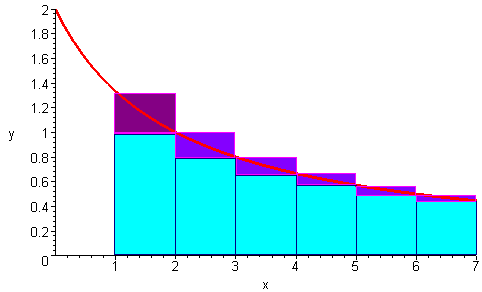
\includegraphics[scale=0.6]{./diagrams/inttes1.png}
  \end{figure}
\end{frame}

\begin{frame}
  \frametitle{Integral Test Exercises}
  Show that the famous harmonic series
  \begin{equation}
    \label{eq:paipawai}
    1+\frac{1}{2}+\frac{1}{3}+\frac{1}{4}+\frac{1}{5}+{\ldots}
  \end{equation}
  diverges. Then show that
  \begin{equation}
    \label{eq:aiphohai}
    1+\frac{1}{2^{2}}+\frac{1}{3^{2}}+\frac{1}{4^{2}}+\frac{1}{5^{2}}+{\ldots}
  \end{equation}
  converges. 
\end{frame}

\begin{frame}
  \frametitle{Integral Test Exercises}
Now show that
  \begin{equation}
    \label{eq:yeefieth}
    \sum_{n=1}^{\infty}\frac{1}{n^{2}+1}
  \end{equation}
  exists. Remember that the antiderivative of
  \begin{equation}
    \label{eq:jaifahti}
    f(x)=\frac{1}{x^{2}+1}
  \end{equation}
is $F(x)=\arctan{}x$. Showing that (\ref{eq:yeefieth}) exists does not
mean that we know its value.
\end{frame}

\begin{frame}
  \frametitle{Integral Test Exercises}
  Give reasons why the following sums exist or do not exist.
  \begin{equation}
    \label{eq:oosuphif}
    \begin{array}{ccccc}
      \displaystyle \sum_{n=1}^{\infty}e^{-n} & \hspace{1in} & \displaystyle \sum_{n=1}^{\infty}\frac{n}{n+1} & \hspace{1in} & \displaystyle \sum_{n=1}^{\infty}n\sin\frac{1}{n} \\
      & \hspace{1in} & \\
      \displaystyle \sum_{n=1}^{\infty}\frac{3}{\sqrt{n}} & \hspace{1in} & \displaystyle \sum_{n=1}^{\infty}\frac{-2}{n\sqrt{n}} & & \displaystyle \sum_{n=1}^{\infty}\frac{n}{n^{2}+1} \\
      & \hspace{1in} & \\
      \displaystyle \sum_{n=2}^{\infty}\frac{\ln{}n}{n} & \hspace{1in} & \displaystyle \sum_{n=1}^{\infty}\frac{5^{n}}{4^{n}+3} & & \displaystyle \sum_{n=2}^{\infty}\frac{\sqrt{n}}{\ln{}n}\\
      % & \hspace{1in} & \\
      % \displaystyle \sum_{n=2}^{\infty}\frac{\sqrt{n}}{\ln{}n} & \hspace{1in} & \displaystyle \sum_{n=1}^{\infty}\frac{1}{(\ln{}3)^{n}} \\
      % & \hspace{1in} & \\
      % \displaystyle \sum_{n=1}^{\infty}n\sin\frac{1}{n} & \hspace{1in} & \displaystyle \sum_{n=1}^{\infty}\frac{n}{n^{2}+1} \\
    \end{array}\notag
  \end{equation}
\end{frame}

\begin{frame}
  \frametitle{Integral Test Answers}
  \begin{equation}
    \label{eq:epeiveix}
    \sum_{n=1}^{\infty}e^{-n}
  \end{equation}
is convergent because it is a geometric series with
$0\leq{}r=\frac{1}{e}<1$.
\begin{equation}
  \label{eq:bauveeze}
\sum_{n=1}^{\infty}\frac{n}{n+1}  
\end{equation}
is divergent because $\frac{n}{n+1}\longrightarrow{}1$, and
$\frac{n}{n+1}\qeq{}0$ implies divergence
according to the $n$-the term test.
\begin{equation}
  \label{eq:uithaezi}
\sum_{n=1}^{\infty}n\sin\frac{1}{n}  
\end{equation}
is divergent because according to L'H{\^o}pital's rule,
$n\sin\frac{1}{n}\longrightarrow{}1$, and $n\sin\frac{1}{n}\qeq{}0$ implies divergence
according to the $n$-the term test.
\end{frame}

\begin{frame}
  \frametitle{Integral Test Answers}
  \begin{equation}
    \label{eq:voomeijo}
\sum_{n=1}^{\infty}\frac{3}{\sqrt{n}}    
\end{equation}
is divergent according to the integral test.
\begin{equation}
  \label{eq:oageevae}
\sum_{n=1}^{\infty}\frac{-2}{n\sqrt{n}}  
\end{equation}
is convergent according to the integral test.
\begin{equation}
  \label{eq:phoewahg}
  \sum_{n=1}^{\infty}\frac{n}{n^{2}+1}
\end{equation}
is divergent because $a_{n}/b_{n}\longrightarrow{}1$ for
$a_{n}=n/(n^{2}+1)$ and $b_{n}=\frac{1}{n}$, using part 1 of the limit
comparison test.
\end{frame}

\begin{frame}
  \frametitle{Integral Test Answers}
  \begin{equation}
    \label{eq:ziegaequ}
    \sum_{n=2}^{\infty}\frac{\ln{}n}{n}
  \end{equation}
  is divergent because $\ln{}n/n>1/n$ for $n>2$ and the harmonic
  series diverges.
  \begin{equation}
    \label{eq:ezahraox}
    \sum_{n=1}^{\infty}\frac{5^{n}}{4^{n}+3}
  \end{equation}
is divergent because $a_{n}/b_{n}\longrightarrow{}1$ for
$a_{n}=5^{n}/(4^{n}+3)$ and $b_{n}=\frac{5^{n}}{4^{n}}$, using part 1 of the limit
comparison test. $\sum{}b_{n}$ diverges because it is a geometric
series with $r>1$.
\begin{equation}
  \label{eq:queiquai}
  \sum_{n=2}^{\infty}\frac{\sqrt{n}}{\ln{}n}
\end{equation}
is divergent because according to L'H{\^o}pital's rule,
$\lim_{x\rightarrow{}\infty}\frac{\sqrt{x}}{\ln{}x}$ does not exist.
\end{frame}

\begin{frame}
  \frametitle{The $n$-th Term Test}
  We could prove this theorem, but it is also accessible to intuition:
  \begin{equation}
    \label{eq:taingaik}
    \mbox{If }\sum_{i=1}^{n}a_{i}\mbox{ converges, then }a_{n}\longrightarrow{}0
  \end{equation}
  \begin{block}{Test for Divergence}
    $\sum_{i=1}^{n}a_{i}$ diverges if $\lim_{n\rightarrow\infty}a_{n}$
    fails to exist or is different from $0$.
  \end{block}
  The converse of the $n$-th term test is not true. For the following
  sequence, the corresponding series diverges even though the sequence
  goes to $0$.
  \begin{equation}
    \label{eq:aephieng}
    1+\underbrace{\frac{1}{2}+\frac{1}{2}}_\text{2 terms}+\underbrace{\frac{1}{4}+\frac{1}{4}+\frac{1}{4}+\frac{1}{4}}_\text{4 terms}+\frac{1}{8}+{\ldots}
  \end{equation}
\end{frame}

\begin{frame}
  \frametitle{Comparison Tests}
  Let $\left(a_{n}\right)_{n\in\mathbb{N}}$ be a sequence with no
  negative terms. Then
  \begin{enumerate}
  \item $\sum{}a_{n}$ converges if there is a convergent series
    $\sum{}c_{n}$ with $a_{n}\leq{}c_{n}$ for all $n>N$, for some
    integer $N$.
  \item $\sum{}a_{n}$ diverges if there is a divergent series
    $\sum{}d_{n}$ with $a_{n}\geq{}d_{n}\geq{}0$ for all $n>N$,
    for some integer $N$.
  \end{enumerate}
\end{frame}

\begin{frame}
  \frametitle{Comparison Test Example}
  \beispiel{Comparison Test Example} The series
  \begin{equation}
    \label{eq:oopoosoo}
    \sum_{n=1}^{\infty}\frac{5}{5n-1}
  \end{equation}
  diverges because
  \begin{equation}
    \label{eq:quaejash}
    \frac{5}{5n-1}=\frac{1}{n-\frac{1}{5}}>\frac{1}{n}
  \end{equation}
for all $n\in\mathbb{N}$.
\end{frame}

\begin{frame}
  \frametitle{Limit Comparison Tests}
  \textbf{1.} If
  \begin{equation}
    \label{eq:eaquaish}
    \lim_{n\rightarrow\infty}\frac{a_{n}}{b_{n}}=c>0
  \end{equation}
then $\sum{}a_{n}$ and $\sum{}b_{n}$ both converge or both
diverge.

\bigskip

  \textbf{2.} If
  \begin{equation}
    \label{eq:ejeixuaj}
    \lim_{n\rightarrow\infty}\frac{a_{n}}{b_{n}}=0
  \end{equation}
and $\sum{}b_{n}$ converges, them $\sum{}a_{n}$ converges.

\bigskip

  \textbf{3.} If
  \begin{equation}
    \label{eq:aeteiroh}
    \lim_{n\rightarrow\infty}\frac{a_{n}}{b_{n}}=\infty
  \end{equation}
and $\sum{}b_{n}$ diverges, them $\sum{}a_{n}$ diverges.
\end{frame}

\begin{frame}
  \frametitle{Ratio Test}
Let $\left(a_{n}\right)_{n\in\mathbb{N}}$ be a sequence with
positive terms and suppose that
\begin{equation}
  \label{eq:lahyaxee}
  \lim_{n\rightarrow\infty}\frac{a_{n+1}}{a_{n}}=\varrho
\end{equation}
Then
\begin{enumerate}
\item the series $\sum{}a_{n}$ converges if $\varrho<1$
\item the series $\sum{}a_{n}$ diverges if $\varrho>1$ or
  $\varrho$ is infinite
\item the test is inconclusive if $\varrho=1$
\end{enumerate}
\end{frame}

\begin{frame}
  \frametitle{Ratio Test Exercises}
  {\ubung} Use the ratio test to find out if the following exist:
  \begin{equation}
    \label{eq:uaxahphe}
    \begin{array}{ccccc}
      \displaystyle \sum_{n=0}^{\infty}\frac{2^{n}+5}{3^{n}} & \hspace{1in} & \displaystyle \sum_{n=1}^{\infty}\frac{(2n)!}{n!n!} & \hspace{1in} & \displaystyle \sum_{n=1}^{\infty}\frac{4^{n}n!n!}{(2n)!} \\
    \end{array}\notag
  \end{equation}
\end{frame}

\begin{frame}
  \frametitle{Leibniz's Theorem}
  Let $\left(u_{n}\right)_{n\in\mathbb{N}}$ be a sequence with
  $u_{n}>0$ for all $n\in\mathbb{N}$. Then
  \begin{equation}
    \label{eq:aegeigho}
    \sum_{n=1}^{\infty}(-1)^{n+1}u_{n}=u_{1}-u_{2}+u_{3}-u_{4}+{\ldots}
  \end{equation}
is an \alert{alternating series}. It converges if the
following two conditions are satisfied:
\begin{enumerate}
\item $u_{n}>u_{n+1}$ for all $n>N$, for some integer $N$
\item $u_{n}\longrightarrow{}0$
\end{enumerate}
It immediately follows that the alternating harmonic series
\begin{equation}
  \label{eq:aighuhif}
  1-\frac{1}{2}+\frac{1}{3}-\frac{1}{4}+\frac{1}{5}-{\ldots}
\end{equation}
converges. It equals $\ln{}2$.
\end{frame}

\begin{frame}
  \frametitle{Harmonic Series}
  An ant starts to crawl along a taut rubber rope 1 km long at a
  speed of 1 cm per second (relative to the rubber it is crawling
  on). At the same time, the rope starts to stretch uniformly by 1
  km per second, so that after 1 second it is 2 km long, after 2
  seconds it is 3 km long, etc. Will the ant ever reach the end of
  the rope? Counterintuitively, yes. This is a consequence of the
  divergent harmonic series.

  \bigskip

  Another example is the block-stacking problem: given a
  collection of identical dominoes, it is clearly possible to
  stack them at the edge of a table so that they hang over the
  edge of the table without falling. The counterintuitive result
  is that one can stack them in such a way as to make the overhang
  arbitrarily large, provided there are enough dominoes.
\end{frame}

\begin{frame}
  \frametitle{Harmonic Series}
  \begin{figure}[h]
    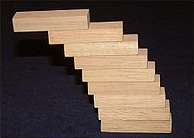
\includegraphics[scale=.02]{./diagrams/harm1.jpg}
  \end{figure}
\end{frame}

\begin{frame}
  \frametitle{Absolute Convergence}
  A series $\sum{}a_{n}$ \alert{converges absolutely} if the
  corresponding series of absolute values $\sum\vert{}a_{n}\vert$
  converges. Are the following two series absolutely convergent?
  \begin{equation}
    \label{eq:pheequie}
    1-\frac{1}{2}+\frac{1}{4}-\frac{1}{8}+\frac{1}{16}-{\ldots}
  \end{equation}
  \begin{equation}
    \label{eq:uaqueigh}
    1-\frac{1}{2}+\frac{1}{3}-\frac{1}{4}+\frac{1}{5}-{\ldots}
  \end{equation}
A series that converges but does not converge absolutely is said
to \alert{converge conditionally}. If $\sum\vert{}a_{n}\vert$
converges, then $\sum{}a_{n}$ must converge. Absolutely (and ONLY
absolutely) convergent series can be rearranged. The alternating
harmonic series can be rearranged to diverge or to reach any
preassigned infinite sum.
\end{frame}

\begin{frame}
  \frametitle{Power Series}
  A \alert{power series about $x=0$} is a series of the form
  \begin{equation}
    \label{eq:eecizaja}
    \sum_{n=0}^{\infty}c_{n}x^{n}=c_{0}+c_{1}x+c_{2}x^{2}+{\ldots}
  \end{equation}
  A \alert{power series about $x=a$} is a series of the form
  \begin{equation}
    \label{eq:coojudie}
    \sum_{n=0}^{\infty}c_{n}(x-a)^{n}=c_{0}+c_{1}(x-a)+c_{2}(x-a)^{2}+{\ldots}
  \end{equation}
in which the centre $a$ and the coefficients $c_{0},c_{1},c_{2}$ are real numbers.
\end{frame}

\begin{frame}
  \frametitle{The Term-by-Term Differentiation Theorem}
  If $\sum_{n=0}^{\infty}c_{n}(x-a)^{n}$ converges for $a-R<x<a+R$ for some $R>0$, it defines a function $f$
  \begin{equation}
    \label{eq:aengooph}
    f(x)=\sum_{n=0}^{\infty}c_{n}(x-a)^{n}\mbox{ on the domain }a-R<x<a+R
  \end{equation}
  Such a function $f$ has derivatives of all orders inside the interval of convergence. We can obtain the derivatives by differentiating the original series term by term.
  \begin{equation}
    \label{eq:eghoocah}
    f'(x)=\sum_{n=1}^{\infty}nc_{n}(x-a)^{n-1}
  \end{equation}
  \begin{equation}
    \label{eq:xalaixii}
    f''(x)=\sum_{n=2}^{\infty}n(n-1)c_{n}(x-a)^{n-2}
  \end{equation}
and so on. Each of these derived series converges at every interior point of the interval of convergence of the original series.
\end{frame}

\begin{frame}
  \frametitle{The Term-by-Term Integration Theorem}
  If $\sum_{n=0}^{\infty}c_{n}(x-a)^{n}$ converges for $a-R<x<a+R$ for some $R>0$, it defines a function $f$
  \begin{equation}
    \label{eq:ohmaekel}
    f(x)=\sum_{n=0}^{\infty}c_{n}(x-a)^{n}\mbox{ on the domain }a-R<x<a+R
  \end{equation}
  Then
  \begin{equation}
    \label{eq:iechaefi}
    \sum_{n=0}^{\infty}c_{n}\frac{(x-a)^{n+1}}{n+1}
  \end{equation}
converges for $a-R<x<a+R$ and
  \begin{equation}
    \label{eq:aibooqui}
    \int{}f(x)\,dx=\sum_{n=0}^{\infty}c_{n}\frac{(x-a)^{n+1}}{n+1}+C
  \end{equation}
for $a-R<x<a+R$.
\end{frame}

\begin{frame}
  \frametitle{First Power Series Expansions}
  Use these two theorems to find power series expansions for $f(x)=\arctan{}x$ and $g(x)=\ln{}(1+x)$ on the domain $-1<x<1$.

  \bigskip

  Use the following two functions to succeed in this endeavour.
  \begin{equation}
    \label{eq:tohpojos}
    f(x)=x-\frac{x^{3}}{3}+\frac{x^{5}}{5}-{\ldots}
  \end{equation}
  \begin{equation}
    \label{eq:queiroxu}
    g(x)=1-x+x^{2}-x^{3}+{\ldots}
  \end{equation}
\end{frame}

\begin{frame}
  \frametitle{The Series Multiplication Theorem for Power Series}
  If $A(x)=\sum_{n=0}^{\infty}a_{n}x^{n}$ and
  $B(x)=\sum_{n=0}^{\infty}b_{n}x^{n}$ converge absolutely for
  $|x|<R$, and
  \begin{equation}
    \label{eq:quewahre}
    c_{n}=a_{0}b_{n}+a_{1}b_{n-1}+{\ldots}+a_{n-1}b_{1}+a_{n}b_{0}=\sum_{k=0}^{n}a_{k}b_{n-k}
  \end{equation}
then $\sum_{n=0}^{\infty}c_{n}x^{n}$ converges absolutely to
$A(x)B(x)$ for $|x|<R$,
\begin{equation}
  \label{eq:axoochid}
  \left(\sum_{n=0}^{\infty}a_{n}x^{n}\right)\cdot\left(\sum_{n=0}^{\infty}b_{n}x^{n}\right)=\sum_{n=0}^{\infty}c_{n}x^{n}
\end{equation}
Use term-by-term differentiation and the series multiplication theorem
for power series independently to show that for $|x|<1$
\begin{equation}
  \label{eq:kahfeipe}
  \frac{1}{(1-x)^{2}}=1+2x+3x^{2}+4x^{3}+{\ldots}
\end{equation}
\end{frame}

\begin{frame}
  \frametitle{Taylor and Mclaurin Series}
  Now think about it the other way around. If a power series gives us
  a continuous function with derivatives of all orders, will a
  continuous function with derivatives of all orders give us a power
  series? What would be the coefficients? Let's assume that
  \begin{equation}
    \label{eq:jeepaipe}
    f(x)=\sum_{n=0}^{\infty}a_{n}(x-a)^{n}
  \end{equation}
  with a positive radius of convergence. 
\end{frame}

\begin{frame}
  \frametitle{Taylor and Mclaurin Series}
Then
  \begin{equation}
    \label{eq:itaivaeg}
    f^{(n)}(x)=n!a_{n}+\mbox{ a sum of terms with }x-a\mbox{ as a factor}
  \end{equation}
  Since these equations all hold at $x=a$, we have
  \begin{equation}
    \label{eq:ahthoazo}
    \begin{array}{rcl}
      f'(a)&=&1\cdot{}a_{1} \\
      f''(a)&=&1\cdot{}2\cdot{}a_{2} \\
      f'''(a)&=&1\cdot{}2\cdot{}3\cdot{}a_{3} \\
    \end{array}
  \end{equation}
    and in general $f^{(n)}=n!a_{n}$.
  \end{frame}

  \begin{frame}
    \frametitle{Taylor and Mclaurin Series}
    So, if (and that's a significant ``if'') a function $f$ has a
    series representation, then the series must be
    \begin{equation}
      \label{eq:ahazohve}
      f(x)=f(a)+f'(a)(x-a)+\frac{f''(a)}{2!}(x-a)^{2}+{\ldots}+\notag
    \end{equation}
    \begin{equation}
      \label{eq:oolietai}
      \frac{f^{(n)}(a)}{n!}(x-a)^{n}+{\ldots}
    \end{equation}
If $f$ is infinitely differentiable, then this series is determined,
but it is not always true that the series has a positive radius of
convergence. All kinds of things can go wrong. For example, the
function
\begin{equation}
  \label{eq:cutailae}
  f(x)=e^{-\frac{1}{x^{2}}}
\end{equation}
has a Mclaurin series which converges everywhere but only at $x=0$
does the limit equal $f(x)$!
  \end{frame}

  \begin{frame}
    \frametitle{Taylor and Mclaurin Series}
    Let $f$ be a function with derivatives of all orders throughout
    some interval containing $a$ as an interior point. Then the
    \alert{Taylor series} generated by $f$ at $x=a$ is
    \begin{equation}
      \label{eq:oetaenis}
      \sum_{k=0}^{\infty}\frac{f^{(k)}(a)}{k!}(x-a)^{k}=f(a)+f'(a)(x-a)+\notag
    \end{equation}
    \begin{equation}
      \label{eq:ikooveiv}
      \frac{f''(a)}{2!}(x-a)^{2}+{\ldots}+\frac{f^{(n)}(a)}{n!}(x-a)^{n}+{\ldots}
    \end{equation}
    The \alert{Mclaurin series} generated by $f$ is
    \begin{equation}
      \label{eq:ohyoobip}
      \sum_{k=0}^{\infty}\frac{f^{(k)}(0)}{k!}(x)^{k}=f(0)+f'(0)(x)+\notag
    \end{equation}
    \begin{equation}
      \label{eq:tolokaav}
      \frac{f''(0)}{2!}(x)^{2}+{\ldots}+\frac{f^{(n)}(0)}{n!}(x)^{n}+{\ldots}
    \end{equation}
  \end{frame}

\begin{frame}
  \frametitle{Taylor and Mclaurin Polynomials}
  When we learned differentiation, we learned about the linear
  approximation of a function $f(x)$ at $x=a$. This linear
  approximation turns out to be the Taylor polynomial of order 1. A
  Taylor polynomial (or Mclaurin polynomial) is a Taylor series with
  the tail cut off. If a function has a Taylor series expansion, you
  can approximate it arbitrarily well with a polynomial as seen on the
  next slide for $\sin(x)$.
\end{frame}

\begin{frame}
  \frametitle{Taylor and Mclaurin Polynomials}
    \begin{figure}[h]
    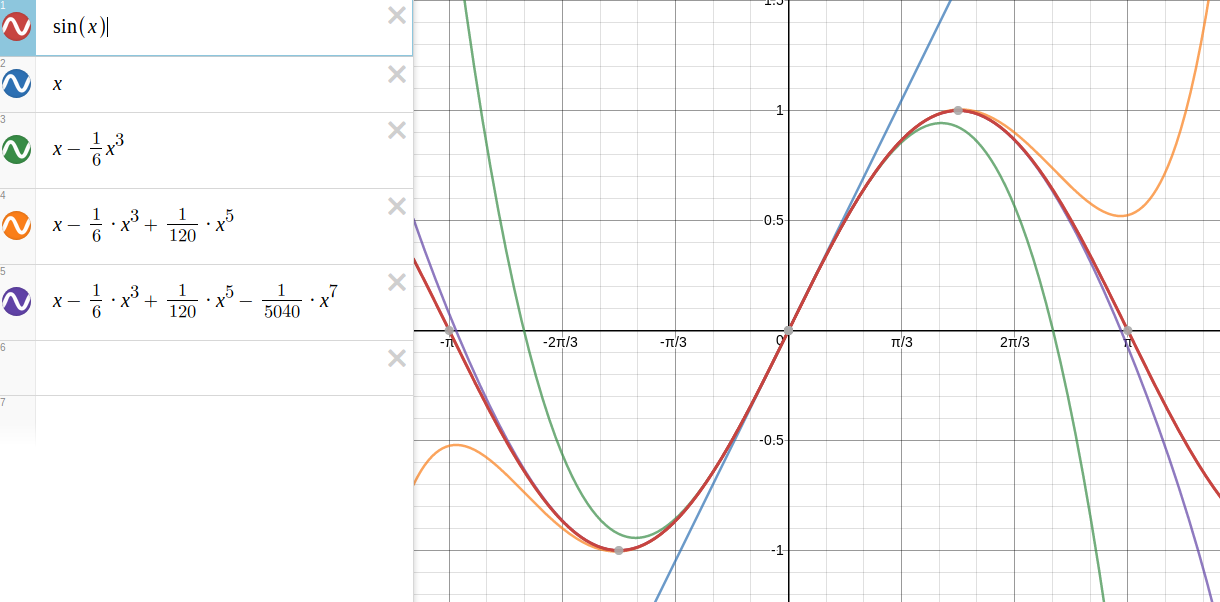
\includegraphics[scale=0.3]{./diagrams/sinappr.png}
  \end{figure}
\end{frame}

  \begin{frame}
    \frametitle{Taylor Series Exercises}
Find the Taylor polynomials of orders 0, 1, 2, 3 generated by $f$
at $a$.
\begin{equation}
\label{eq:chaithie}
f(x)=\ln{}x,\;a=1
\end{equation}
\begin{equation}
\label{eq:oorohkao}
f(x)=\frac{1}{x},\;a=2
\end{equation}
\begin{equation}
\label{eq:foigacoo}
f(x)=\sin{}x,\;a=\frac{\pi}{4}
\end{equation}
\begin{equation}
\label{eq:sishahgh}
f(x)=\sqrt{x},\;a=4
\end{equation}
\begin{equation}
  \label{eq:eighetog}
f(x)=\cos{}x,\;a=\frac{\pi}{4}
\end{equation}
\end{frame}

\begin{frame}
  \frametitle{Mclaurin Series Exercises}
  Find the Mclaurin series for the following functions.
  \begin{equation}
    \label{eq:oxishait}
    f(x)=e^{-x}
  \end{equation}
  \begin{equation}
    \label{eq:chuyeeye}
    f(x)=e^{\frac{x}{2}}
  \end{equation}
  \begin{equation}
    \label{eq:queiyuif}
    f(x)=\frac{1}{1+x}
  \end{equation}
  \begin{equation}
    \label{eq:aoyahphe}
    f(x)=\cosh{}x
  \end{equation}
  \begin{equation}
    \label{eq:ahtoilei}
    f(x)=\sinh{}x
  \end{equation}
\end{frame}

\begin{frame}
  \frametitle{End of Lesson}
Next Lesson: Multivariable Calculus
\end{frame}

\end{document}

